\begin{figure}[t]
\centering
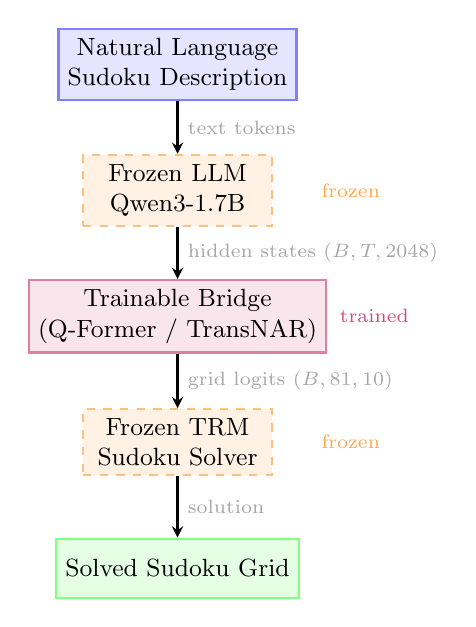
\begin{tikzpicture}[
    box/.style={rectangle, draw, thick, minimum width=2.4cm, minimum height=0.75cm, align=center, font=\small},
    input/.style={box, fill=blue!10, draw=blue!50},
    frozen/.style={box, fill=orange!10, draw=orange!50, dashed},
    bridge/.style={box, fill=purple!10, draw=purple!50},
    output/.style={box, fill=green!10, draw=green!50},
    arrow/.style={->, >=stealth, thick},
    label/.style={font=\scriptsize, color=gray!70}
]

% Nodes
\node[input]  (inp)    at (0,    0) {Natural Language\\Sudoku Description};
\node[frozen] (llm)    at (0,   -1.6) {Frozen LLM\\Qwen3-1.7B};
\node[bridge] (bridge) at (0,   -3.2) {Trainable Bridge\\(Q-Former / TransNAR)};
\node[frozen] (trm)    at (0,   -4.8) {Frozen TRM\\Sudoku Solver};
\node[output] (out)    at (0,   -6.4) {Solved Sudoku Grid};

% Arrows
\draw[arrow] (inp)    -- node[right, label] {text tokens} (llm);
\draw[arrow] (llm)    -- node[right, label] {hidden states $(B,T,2048)$} (bridge);
\draw[arrow] (bridge) -- node[right, label] {grid logits $(B,81,10)$} (trm);
\draw[arrow] (trm)    -- node[right, label] {solution} (out);

% Frozen annotation
\node[label, color=orange!70, align=left] at (2.2, -1.6) {frozen};
\node[label, color=orange!70, align=left] at (2.2, -4.8) {frozen};
\node[label, color=purple!70, align=left] at (2.5, -3.2) {trained};

\end{tikzpicture}
\caption{Pipeline overview. A frozen LLM encodes a natural-language Sudoku description; a trainable bridge maps hidden states to a grid; a frozen TRM solves the puzzle. Only the bridge is trained.}
\label{fig:sudoku_pipeline}
\end{figure}
